\documentclass[oneside,senior,etd]{BYUPhys}

\usepackage[utf8]{inputenc}
\usepackage{rotating} 

\usepackage[english, russian]{babel}
\usepackage{amsfonts} % Пакеты для математических символов и теорем
\usepackage{amstext}
\usepackage{amssymb}
\usepackage{amsthm}
\usepackage{graphicx} % Пакеты для вставки графики
\usepackage{subfig}
\usepackage{color}
\usepackage[unicode]{hyperref} 
\usepackage[nottoc]{tocbibind} % Для того, чтобы список литературы отображался в оглавлении
\usepackage{algorithmic} % Для записи алгоритмов в псевдокоде
\usepackage{algorithm}
\usepackage{verbatim} % Для вставок заранее подготовленного текста в режиме as-is
\usepackage{indentfirst}

\usepackage{tikz} 
\usetikzlibrary{positioning}
\usetikzlibrary{shadows,arrows}

\Chair{Кафедра информационной безопасности}
\Lab{~}
\Year{2018}
  \Month{}
  \City{Москва}
  \AuthorText{}
  \Author{}
  \AuthorEng{}
  \AcadGroup{}

  \TitleTop{Разработка итерационных алгоритмов поиска автоморфизмов}
  \TitleBottom{и изоморфизмов комбинаторных объектов.} % leave empty if you don't need it
  \TitleName{ВЫПУСКНАЯ КВАЛИФИКАЦИОННАЯ РАБОТА}
  \TitleTopEng{Development of iterative algorithms for searching}
  \TitleBottomEng{automorphisms and isomorphisms of combinatorial objects.} % leave empty if you don't need it  
  \docname{Ефремов Степан Сергеевич}
  \Advisor{
  
  Егоров Владимир Николаевич}  
  \AdvisorDegree{доцент, к.ф.- м.н.}



%%%% DON'T change this. It is here because .sty does not support cyrillic cp properly %%%%
\University{Московский государственный университет имени М.В.Ломоносова}
\Faculty{Факультет вычислительной математики и кибернетики}
\GrText{группа}
\AdvisorText{Научный руководитель}

\begin{document}
\fixmargins
\makepreliminarypages

\oneandhalfspace

\tableofcontents

\newtheorem{statement}{Гипотеза}

\section*{Аннотация}
\addcontentsline{toc}{section}{Аннотация}
\label{sec:Annotation} \index{Annotation}
\large

Дипломная работа разбита на следующие пункты:
\begin{enumerate}
\item Постановка задачи: сформулированы задачи дипломной работы.
\item Основные определения и обозначения: приводятся основные понятия, используемые в ходе работы.
\item Структура алгоритма: описывается алгоритм из статьи.
\item Исследование алгоритма: в данном пункте описан класс решаемых задач алгоритмом, полученны оценки сложности. А также определены способы модернизации, которые удалось найти в ходе исследования. Особое внимание уделяется исследованию расспараллеливания вычислений программной реализации.
\item Модернизация алгоритма: описаны все найденные способы модернизации.
\item Практическое применение: рассказывается о различных применениях разработанного алгоритма для графов и некоторых других комбинаторных объектов. В том числе, рассматриваются способы использования алгоритма для задачи Коши.
\item Разработка программных модулей: рассматриваются ключевые моменты, на которые уделялось особое внимание при реализации програмных модулей. В результате получены 2 программы: упрощенный вариант с графическим интерфейсом для использования на графах с небольшим количеством вершин; вариант реализации для суперкомьпютеров для более удобного сбора информации и исследования эффективности.
\item Результаты опробывания программ: в этом пункте приводится анализ результатов, полученных при тестировании разработанных программ на различных данных, также подробно проанализированы результаты запусков программы на суперкомьпьютере Ломоносов.
\end{enumerate} % аннотация
\section*{Введение}
\addcontentsline{toc}{section}{Введение}
\label{sec:Introduction} \index{Introduction}
\large 

Проблема изоморфизма графов в настоящее время приобрела статус одной из самых сложных и важных с теоретической точки зрения задач комбинаторной математики. Известно, что решение задачи нахождения изоморфного подграфа с точки зрения алгоритмической сложности позволило бы ответить на вопрос о совпадении или различии классов P и NP. В последние годы сформировались два направления изучения и решения данной проблемы. Первое направление - теоретическое, в котором проблема изоморфизма рассматривается с позиций соременной теории сложности алгоритмов и вычислений, а второе - сугубо практическое, предполагающее разработку алгоритмов, решающих задачу изоморфизма графов за "практически приемлемое" время.

Первые серьёзные результаты в теоретическом направлении появились в 50-х и 60-х годах прошлого века. Для нескольких семейств графов была установлена полиномиальная сложность нахождения изоморфизма. В 70-х годах, особенно после выхода в свет замечательной монографии Нормана Биггса "Алгебраическая теория графов", к решению этой задачи подключились крупные специалисты в области линейной алгебры, теории групп и ряда других направлений общей алгебры. Результаты не замедлили сказаться - открыто много новых интересных алгебраических свойств графов. В 1979 году Егорову В.Н. удалось получить положительное решение гипотезы Адама об изоморфизме графов с циркулянтными матрицами смежности вершин порядка свободного от квадратов [1].
В дипломной работе рассматривается итерационный алгоритм поиска автоморфизмов и изоморфизмов графов.

Поиск автоморфизмов и изоморфизмов алгебраических систем, в том числе графов, является известной задачей. Опубликовано множество книг и научных статей, посвященных данной проблеме. Из существующих алгоритмов на данный момент стоит выделить "кратко об алг. Лакса (про ограниченную Валентность)"{}, "кратко об алг. в случае циркулянтной матрицы смежности"{}.

Как выяснилось, эффективного (полиномиального) алгоритма, который был бы универсальным, т.е. применим к любым графам, сейчас не существует. На основании этого было решено исследовать итерационный алгоритм, предложенный в статье В.Н.Егорова [1].

Работа разбита на следующие пункты:
\begin{enumerate}
\item Постановка задачи.
\item Основные определения и обозначения: приводятся основные понятия, используемые в ходе работы.
\item Структура алгоритма.
\item Исследование и модернизация алгоритма: в данном пункте описаны полученные оценки сложности алгоритма, а также способы модернизации, которые удалось найти в ходе исследования. Особое внимание уделяется исследованию расспараллеливания вычислений программной реализации.
\item Практическое применение: рассказывается о различных применениях алгоритма для графов и некоторых других комбинаторных объектов. В том числе, рассматриваются способы использования алгоритма для задачи Коши.
\item Разработка программных модулей: рассматриваются ключевые моменты, на которые стоило уделить особое внимание при реализации програмных продуктов. В результате получены 2 программы: упрощенный вариант с графическим интерфейсом для использования на графах с небольшим количеством вершин; вариант реализации со всеми модернизациями, упомянутыми во 2-ом пункте, для более удобного сбора информации и исследования эффективности.
\item Результаты опробывания программ: в этом пункте приводится анализ результатов, полученных при тестировании разработанных программ на различных данных, также подробно проанализированы результаты запусков программы на суперкомьпьютере Ломоносов.
\end{enumerate} % введение
\section{Постановка задачи}
\label{sec:Problem_1} \index{Problem_1}
\large

Целью данной работы является:
\begin{enumerate}
\item Исследование свойств алгоритма:
\begin{itemize}
\item Определение класса решаемых задач
\item Вероятностная сложность
\item Теоретическая возможность распараллеливания
\item Модернизация алгоритма на основе исследований
\end{itemize}
\item Задачи, связанные с реализацией для ПК:
\begin{itemize}
\item Реализация в виде программы с графическим интерфейсом
\item Эксперименты поиска автоморфизмов на известных графах
\item Поддержа функционала нахождения изоморфного вложения графов
\end{itemize}
\item Задачи, связанные с реализацией для суперкомпьютера:
\begin{itemize}
\item Исследование ресурса параллелизма
\item Реализация в виде программы для запуска на суперкомпьютере
\item Эксперименты поиска автоморфизмов графов на суперкомпьютере
\end{itemize}
\item Исследование практического применения алгоритма для задачи Коши
\end{enumerate}

 % постановка задачи
\section{Основные определения и обозначения}
\label{sec:Definition_2} \index{Definition_2}
\large

\subsection{Определения}

В работе часто упоминается понятие изоморфизма графов, которое описано ниже. В общем случае, \textbf{изоморфизм} можно описать так: обратимое отображение (биекция) между двумя множествами, наделёнными структурой, называется изоморфизмом, если оно сохраняет эту структуру.

\begin{itemize}
\item \textbf{Автоморфизм алгебраической системы} -- изоморфизм, отображающий алгебраическую систему на себя.

\item \textbf{Автоморфизм графа} -- отображение множества вершин на себя, сохраняющее смежность.

\item \textbf{\mathversion{bold} Изоморфизм графов $G=\left\langle V_{G},E_{G}\right\rangle$ и $H=\left\langle V_{H},E_{H}\right\rangle$} -- биекция между множествами вершин графов $f\colon \ V_{G}\rightarrow V_{H}$ такая, что любые две вершины $u$ и $v$ графа $G$ смежны тогда и только тогда, когда вершины $f(u)$ и $f(v)$ смежны в графе $H$.

\item \textbf{\mathversion{bold} Матрица смежности графа $G$} -- квадратная матрица $A$ размера $n$, в которой значение элемента $a_{ij}$ равно числу рёбер из $i$-й вершины графа в $j$-ю вершину.

\item \textbf{Инвариант графа} -- некоторое числовое значение или упорядоченный набор значений (хэш-функция), характеризующее структуру графа $ G=\langle A,V\rangle $  и не зависящее от способа обозначения вершин или графического изображения графа.

\item \textbf{Регулярный (однороодный) граф} -- граф, степени всех вершин которого равны, то есть каждая вершина имеет одинаковое количество соседей.

\item \textbf{\mathversion{bold} Cильно регулярный граф $srg(v, k, \lambda, \mu)$} -- регулярный граф $G=\left\langle V_{G},E_{G}\right\rangle$ с $v$ вершинами и степенью $k$, для которого существуют целые $\lambda$ и $\mu$ такие, что:
\begin{enumerate}
\item Любые две смежные вершины имеют $\lambda$ общих соседей.
\item Любые две несмежные вершины имеют $\mu$ общих соседей.
\end{enumerate}




\end{itemize}




\subsection{Обозначения}

\begin{itemize}
\item \textbf{\mathversion{bold} $A = A^{n\times n}$} -- матрица смежности графа $G(V,E)$ размера $n\times n$ с элементами $a_{ij}$, $\ i,j = 1,\ldots,n=|V|$.

\item \textbf{\mathversion{bold} $f(u) = v$} -- отображение вершины $u$ в вершину $v$.

\item \textbf{\mathversion{bold} Подстановка изоморфизма $g_n$} -- биекция $f$ вида:

\[ 
    \begin{pmatrix}
    {
		u_1 & u_2 & \ldots & u_n \cr
		f(u_1) & f(u_2) & \ldots & f(u_n) 
	}
    \end{pmatrix}
\]

\item \textbf{\mathversion{bold} Частичная подстановка изоморфизма $g_k$ (частичное отображение)} -- подстановка вида: 

\[
    \begin{pmatrix}
    {
		u_1 & u_2 & \ldots & u_k \cr
		f(u_1) & f(u_2) & \ldots & f(u_k)
    }
    \end{pmatrix}
\]

, где $k \leq n$.
%, где $r_1,\ldots,r_k$ - фиксированные (заданные) элементы, $q_{k+1},\ldots,q_n$ - произвольные, причем последовательность $r_1,\ldots,r_k$, $q_{k+1},\ldots,q_n$ является перестановкой вершин заданного графа.

\item \textbf{\mathversion{bold} $\widehat{g}$} -- матричный вид подстановки $g$.

\item \textbf{\mathversion{bold} $\widehat{g} A \widehat{g}^{-1} = A$} -- автоморфизм графа $A$.

\item \textbf{\mathversion{bold} $\widehat{g} A \widehat{g}^{-1} = B$} -- изоморфность графов $A$ и $B$.

\item \textbf{\mathversion{bold} $M_k$} -- множество, состоящее из элементов $g^s_k$, $\ s = 1,\ldots,m_k=|M_k|$. 

\item \textbf{\mathversion{bold} $|M_k|$} -- количество элементов множества $M_k$.

\item \textbf{\mathversion{bold} $M'_k$} -- множество элементов, которые содержатся в $M_k$ и удовлетворяют определенному критерию.

\item \textbf{\mathversion{bold} $\{M'_k\}$} -- последовательность множеств $M'_k$, $k = 1,\ldots,n$. 
\end{itemize}


 % определения и обозначения
\section{Структура алгоритма}
\label{sec:AlgoStruct_3} \index{AlgoStruct_3}
\large

\subsection{Входные данные}

На вход алгоритму подается матрица смежности $A^{n \times n}$ графа $G(V,E)$, $n = |V|$.

\subsection{Процедура построения множеств частичных отображений}

Для матрицы $A$ размера $n \times n$ строится последовательность множеств частичных отображений ${M'_n}$ следующим образом. $M_0 = M'_0 = \{g_0\}$, $g_0$ - пустая подстановка. Для всех $i = 1 \ldots n$:
\begin{enumerate}
\item Фиксируем подматрицу $A_i$ размера $i \times i$.

\item Строим множество $M_i$:
\begin{enumerate}
\item Рассматриваем все возможные частичные подстановки $g_i$, полученные из подстановок $g^s_{i-1}$ путем добавления в них отображения $f(u_i) = v_l$.
\item Генерируем множество $M_i$ из подстановок $g_i$, для которых в отображении $f(u_i) = v_l$:
$$l \in \{l\ |\ v_l \neq f(u_j), j = 1 \ldots i-1\}$$
\end{enumerate}

\item Строим множество $M'_i$ (для этого убираем из множества $M_i$ элементы $g_i$, которые не удовлетворяют критерию):
\begin{enumerate}
\item Применяем частичные подстановки к матрице $A$ по отдельности: $\widehat{g_i}A\widehat{g_i}^{-1} = A^{i \times i}_{g_i}$.
\item Генерируем множество $M'_i$ из частичных подстановок, для которых выполнено: $A^{i \times i}_{i} = A^{i \times i}_{g_i}$.
\end{enumerate}

\item Если $i = n$, процедура завершена.
\end{enumerate}



Таким образом, получается последовательнось множеств частичных отображений:

$$\{M'_k\}: M'_1 \supseteq M'_2 \supseteq \ldots \supseteq M'_n$$.

Множество $M'_n$ является множеством всех возможных частичных подстановок $g_n$ длины $n$, то есть всех подстановок изоморфизма графа $G$ на себя. Следовательно $M'_n$ содержит все автоморфизмы.


\subsection{Выходные данные}

Множество подстановок изоморфизма $g^s_n$ графа $G$ на себя (автоморфизмы).
Для всех $s = 1, \ldots ,|M'_n|$, $g^s_n$ имеет вид:

\[ 
    \begin{pmatrix}
    {
		u_1 & u_2 & \ldots & u_n \cr
		f_s(u_1) & f_s(u_2) & \ldots & f_s(u_n) 
	}
    \end{pmatrix}
\]

\subsection{Примечания к процедуре}

В случае задачи определения изоморфизма (или гомоморфизма) графов на вход падается матрица смежности $A^{n \times n}$ и матрица смежности $B^{m \times m}$. Не ограничивая общности считаем, что $n \geq m$. Тогда отличия в процедуре следующие:

\begin{itemize}
\item Случай изоморфизма: вместо подматрицы $A_i$ используется подматрица $B_i$.

\item Случай гомоморфизма: вместо подматрицы $A_i$ используется подматрица $B_i$. Процедура завершается при $i = m$.
\end{itemize}


Критерием $h$ является проверка подматриц на равенство. Предположим, требуется определить, удовлетворяет ли элемент $g^s_k$ критерию. Для этого необходимо, чтобы элементы $a_{ij}$, для всех $i,j \leq k$, были равны соответствующим элементам $a_{r_ir_j}$. Подматрица $\widehat{g^s_k}A\widehat{g^s_k}^{-1} = A_{g^s_k}$ выглядит так:

\[ \bordermatrix{
& r_1 & r_2 & \dots & r_k \cr
r_1 & a_{r_1r_1} & a_{r_1r_2} & \dots & a_{r_1r_k} \cr
r_2 & a_{r_2r_1} & a'_{r_2r_2} & \dots & a_{r_2r_k} \cr
\vdots & \vdots & \vdots & \ddots & \vdots \cr
r_k & a_{r_kr_1} & a_{r_kr_2} & \dots & a_{r_kr_k} \cr}
\]

Если хотя бы одно из равенств не выполнено, это означает, что после применения частичной подстановки к $A$ подматрица $A_i$ не совпадает с $A_{g^s_k}$. Но добавление отображения в частичную подстановку не изменяют подматрицу $A_{g^s_k}$, следовательно для $g^s_n$ образованной от $g^s_k$ $A_n \neq A_{g^s_n}$, ни для какого $s$. Это значит, что частичную подстановку $g^s_k$ можно не рассматривать.


 % описание алгоритма
\section{Исследование алгоритма}
\label{sec:AlgoResearch_4} \index{AlgoResearch_4}
\large


\subsection{Определение класса решаемых задач}
Предложенный алгоритм является универсальным. Используя различный формат вводимых данных, можно решать следующие задачи:
\begin{enumerate}
\item Нахождение группы автоморфизмов произвольной квадратной матрицы.
\item Нахождение левой и правой групп автоморфизомв произваольной матрицы (т.е. блок-схем, дискретных функций и т.д.).
\item Нахождение всех изоморфизмов матрицы $A$ на матрицу $B$.
\item Нахождение всех изоморфных вложений матрицы $A$ в матрицу $B$.
\item Поиск клик.
\item Решение задачи Коши в подстановках.
\item Нахождение группы автоморфизмов матрицы Адамара.
\item Нахождение всех изоморфизмов кода $A$ на код $B$.
\end{enumerate}

В рамках дипломной работы рассматриваются первые шесть задач.

\subsection{Анализ}

Алгоритм применим для любых графов, но для удобства рассматриваются случайные графы, матрицы смежности которых состоят из нулей и единиц.
В этом случае получена оценка сложности алгоритма в среднем.

Так как граф случайный, элементы матрицы смежности графа равны $1$ или $0$ с вероятностью $\frac{1}{2}$. Необходимо вычислить наиболее вероятные размеры для каждого множества $M'_k$.

Если рассмотреть построение множеств, не учитывая промежуточного критерия, то на $k$-ом шаге множество увеличивается \ в $(n-k)$ раз (так как для каждого элемента $g^s_{(k-1)} = (r_1, \ldots, r_{k-1})$ добавляется $r_k$ из оставшихся $(n-k)$ вариантов): $|M_{k+1}| = |M_{k}|(n-k)= n(n-1)\ldots(n-k)$.

С учетом критерия получается:

\begin{enumerate}
\item Из построения множества $M'_1$ следует $|M'_1|\thickapprox\frac{|M_1|}{2}$ (элемент $a_{11}$ = $a_{r_1r_1}$ с вероятностью $\frac{1}{2}$).
\item На $(k+1)$-ом шаге требуется совпадение $((k+1) + (k+1) - 1)$ элементов. Так как граф случайный (матрица с равновероятным распределением $0$ и $1$), то на этом шаге $|M'_{k+1}| = \frac{1}{2^{2m+1}}|M_k|$ элементов.
\end{enumerate}

 Учитывая построение $\{M'_k\}$ и пункты 1, 2 получим
 
 $|M'_{k+1}| \thickapprox \frac{n!}{(n-k-1)!~2^{(k+1)^2}} \thickapprox \frac{1}{e^{k+1}} \frac{n^{n+1/2}}{(n-k-1)^{(n-k-1/2)}~2^{(k+1)^2}}$. Последнее равенство получено используя формулу Стирлинга: $n!\thickapprox \sqrt{2\pi n}(\frac{n}{e})^n$, при большом $n$.
 


Далее необходимо рассмотреть последовательность $\{|M'_{k+1}|\}$. 

$|M'_{k+1}| = \frac{n(n-1)\ldots(n-k)}{2^{(k+1)^2}} \le \frac{n^{k+1}}{2^{(k+1)^2}}$

Равенство $n^{k+1} = 2^{(k+1)^2}$ означает, что в множестве осталось небольшое количество элементов. Данное равенство далее будет называться стабилизацией последовательности $\{M'_k\}$, а $k$ - значением стабилизации.

После решения данного равенства, получается, что стабилизация наступает при $k \thickapprox \log _2(n) $.
Это означает, что с вероятностью близкой к единице (для случайного графа) уже на $k = \lceil\log _2(n) \rceil$ шаге мы обнаружим отсутствие или наличие автоморфизма (в статье это выдвигается как тезис).

Вычисление номера множества $k$ в последовательности $\{|M'_{k}|\}$, соответствующий самому большому множеству:

Пусть $|M'_{k+1}|:$ $|M'_{k+1}| = f(k+1)$, 

$f'(k+1) = \frac{\ln(n)n^{k+1}2^{(k+1)^2}-(2k+2)\ln(2)2^{(k+1)^2}n^{k+1}}{(2^{(m+1)^2})^2}$. 

Получается уравнение:

$\ln(n) - (2k+2)\ln(2) = 0\ \Rrightarrow \  k+1 \thickapprox \frac{5}{7}\ln(n) - 1$. 

Так как $k$ и $n$ целые, то 

$k + 1 = \lceil(\frac{5}{7}\ln(n) - 1)\rceil)$.

Необходимо отметить, что в тот момент, когда $k \thickapprox \log _2(n)$, можно судить о том, существуют автоморфизмы в графе или нет. Если размер множества $M_k = 1$ (только тождественная подстановка), можно утверждать с вероятностью близкой к 1, что автоморфизмов, кроме тривиальной подстановки, не существует. Если $M_k > 1$, то, наоборот, с вероятностью близкой к 1 автоморфизм существует. Данный факт позволяет сэкономить память и уменьшить количество операций при поиске автоморфизмов в тех графах, в которых они существуют.

Опираясь на вышесказанное, получены оценки:
\begin{itemize}
\item значение стабилизации 

$k \thickapprox \log _2(n)$
\item номер наибольшего по количеству элементов множества 

$k \thickapprox \frac{5}{7}\ln(n)$
\item ограничение на размер множества 

$|M'_k| = \frac{n(n-1)\ldots(n-k-1)}{2^{(k)^2}} \le \frac{n^{k}}{2^{(k)^2}}$
\item приблизительное количество операций в секунду:

$\frac{n^{(5/7) \ln(n)}}{2^{((5/7)\ln(n))^2}}\times n(2(\frac{5}{7}\ln(n)) + 1)\times \log_2(n)$

\item затраты оперативной памяти: 

$2 \times \frac{n^{(5/7) \ln(n)}}{2^{((5/7)\ln(n))^2}} \times \log_2(n)$
\end{itemize}

\subsection{Вероятностная сложность}

Сложность всего алгоритма представляет собой сумму сложностей вычисления $M'_1 \ldots M'_n$.

Количество элементов в каждом множестве (с вероятностью близкой к единице):

$ |M'_{k}| \thickapprox \frac{n!}{(n-k-2)!~2^{(k)^2}} \thickapprox \frac{1}{e^{k}} \frac{n^{n+1/2}}{(n-k-2)^{(n-k-3/2)}~2^{(k)^2}} $

Можно оценить: $ |M'_k| = \frac{n(n-1)\ldots(n-k-1)}{2^{(k)^2}} \le \frac{n^{k}}{2^{(k)^2}} $

Количество операций сравнения для подсчета всех множеств:

$ \sum_{k = 1}^{n} \frac{1}{e^{k}} \frac{n^{n+1/2}}{(n-k-2)^{(n-k-3/2)}~2^{(k)^2}} \times (n - k)(2k + 1)$

Оценка (были учтены точка стабилизации и точка максимума последовательности множеств):

$ n \times \frac{n^{(5/7) \ln(n)}}{2^{((5/7)\ln(n))^2}}\times n(2(\frac{5}{7}\ln(n)) + 1)\times \log_2(n) = O(n^2(\frac{e}{2})^{\ln(n)^2} \ln(n))$

Сложность субэкспоненциальная.

\begin{statement}
Асимптотическая сложность алгоритма для случайного графа, выраженная в количестве операций:

$$O(n^2(\frac{e}{2})^{\ln(n)^2} \ln(n))$$

с вероятностью $p$: $p \to 1$, при $n \to \infty$.
\end{statement}

\subsection{Теоретическая возможность распараллеливания}

Каждое множество $ M_i (i = 2 \ldots n) $ вычисляется из $ M'_{i-1} $ путем добавления в каждый элемент (частичная перестановка, представленная вектором целых чисел) из $ M'_{i-1} $ всех возможных оставшихся чисел, которых нет в соответствующем элементе.

Для этого удобно использовать 2 не фиксированных по количеству строк двумерных массива размера t на n (t может увеличиваться), хранящих частичные отображения, такого вида: 

\[
\begin{pmatrix}
{
a_{11} & a_{12} & \ldots &a_{1i} & ? & \ldots & ? \cr
a_{21} & a_{22} & \ldots &a_{2i} & ? & \ldots & ? \cr \ldots \cr
a_{k1} & a_{k2} & \ldots &a_{ki} & ? & \ldots & ? \cr
?      & ?      & \ldots &   ?   & ? & \ldots & ? \cr
\ldots \cr
?      & ?      & \ldots &   ?   & ? & \ldots & ? \cr
}
\end{pmatrix}
\]

? - эти значения не известны и заполняются постепенно.

Один массив для $ M'_{i-1} $, другой для вычисления из предыдущего $ M_i $.
Из каждой строки множества $ M'_{i-1} $ (первый массив), в соответствие с алгоритмом, получается $ n $ новых строк длины i, которые записываются во второй массив (расширяется, если нужно).

После этого, второй массив копируется в первый и запускается цикл по всем векторам. Вектор исключается из массива, если $ a_{ji} $ равен какому-либо числу в данном векторе или вектор с $ a_{ji} $ является частичной перестановкой, не удовлетворяющей критерию.
 % исследование алгоритма 
\section{Модернизация}
\label{sec:AlgoModern_5} \index{AlgoModern_5}
\large

\subsection{Оптимизация по времени работы}
На основе результатов тестирования программы и анализа выяснилось, что эффективность алгоритма тесно связана с тем, как нумеруются вершины графа. Другими словами, время работы программы зависит от того, какой матрицей смежности (из многих) представляется граф.

Модернизация заключается в том, что на каждом этапе можно требовать, чтобы мощность множества частичных отображений была минимальна. Однако представить матрицу смежности нужным образом не представляется возможным при больших размерах, и время работы, затрачеваемой на это, превышает время работы алгоритма. Например, при $n = 100$ потребуется всего лишь 100 операций, чтобы выяснить, с какой вершины эффективнее всего начать отсчет на первой итерации. Но для того, чтобы получить выгоду на второй итерации, уже требуется более 10 000 операций [3]. Поэтому оптимальным является уменьшить только начальное множество частичных отображений.

Для получения первого множества, мощность которого будет наименьшей, в
изначальной матрице меняется порядок строк/столбцов (переименование вершин), а
именно, необходимо поменять строки и соответствующие им столбцы таким образом,
чтобы на месте первого элемента главной диагонали стояло то значение, которое встречается меньше всех других на диагонали. То есть, если на главной диагонали $70\%$ нулей и $30\%$ единиц,
необходимо поместить на первую позицию единицу. Эффективность данной модификации
исходит из того, что первая итерация алгоритма составляет множество из тех номеров
строк (столбцов), в которых значение на главной диагонали совпадает с первым
элементом главной диагонали. Значит, выбрав на эту позицию наименьший по количеству встречаний на диагонали
элемент, получается наименьшее по мощности множество.

Оценки получены для случайных матриц (вероятность нуля и единицы в каждой позиции
одинакова и равна $\frac{1}{2}$).
Предположим, что в матрице $n\times n$ на главной диагонали находится $k$ нулей, где $k \leq \frac{1}{2} n$ (если количество нулей больше половины, то за $k$ обозначается количество единиц).
Тогда, если на первое место главной диагонали выбирать элемент случайным образом,
получим, что математическое ожидание размера полученного множества будет $\frac{k}{n}*k + \frac{n-k}{n}*(n-k)$.
В модифицированном алгоритме всегда будет получаться $k$. Таким образом,
улучшение составляет $\frac{\frac{k}{n} * k + \frac{(n-k)}{n} * (n-k)} {k} = 2 \frac{k}{n} + \frac{n}{k} - 2$ раз. В случае диагонали,
состоящей из одних нулей (единиц), то есть k = 0, улучшение равняется 1 (мнощьность
множеств одинакова).
Для получения полной оценки необходимо посчитать матожидание улучшения для
произвольного числа нулей и единиц на главной диагонали. Вероятноть $k$ нулей
составляет $\frac{C_n^k}{2^n}$. Тогда матожидание улучшения $\frac{1}{2^{n-1}} + 2 \sum\limits_{i=1}^{\lceil\frac{n}{2}\rceil} \frac{C_n^k}{2^n} * (2\frac{k}{n} + \frac{n}{k} - 2)$.
Далее в таблице приведены значения для различных $n$:

\begin{tabular}[t]{||l|l||}
\hline
Количество вершин графа & Коэф. уменьшения мощности \\
\hline
4 &  2.12500 \\
\hline
8 & 2.11198 \\
\hline
14 & 1.69565 \\
\hline
20 & 1.51723 \\
\hline
50 & 1.27697 \\
\hline
100 & 1.18312 \\
\hline
200 & 1.12400 \\
\hline
\end{tabular}

\subsection{Обработка особых случаев}
Из описания алгоритма следует: если в начале построения последовательности множеств частичных отображений, множества имееют размер $\approx n \times (n-1) \times \ldots \times i$ для нескольких $M'_i$, то возможны 2 случая:

\begin{enumerate}
\item Граф действительно имеет много автоморфизмов, в этом случае работа алгоритма будет занимать большее время, чем обычно 

\item Матрица смежности алгоритма оказалась не совсем удобной для использования, в этом случае, можно просто выбрать случайную другую матрицу смежности (например, случай двудольного графа)
\end{enumerate} 

\subsection{Ресурс параллелизма}
Для поиска автоморфизмов матрицы порядка $n$ итерационным алгоритмом в параллельном варианте требуется выполнить:

\begin{itemize}
\item $n$ ярусов сравнений (количество сравнений $ k = 1 \ldots n: \frac{1}{e^{k}} \frac{n^{n+1/2}}{(n-k-2)^{(n-k-3/2)}~2^{(k)^2}} \times (n - k)(2k + 1) $)
\end{itemize}

При классификации по высоте ЯПФ, таким образом, алгоритм имеет сложность $ O(n) $.

При классификации по ширине ЯПФ его сложность $ O(n(\frac{e}{2})^{\ln(n)^2} \ln(n))) $.
 % модернизация алгоритма
\section{Практическое применение}
\label{sec:AlgoPractice_6} \index{AlgoPractice_6}
\large

Разработанный алгоритм является универсальным и может применяться для решения большого количества задач (как минимум всех указанных в пункте 4.1).

Написанная программа с интерфейсом имеет масштабируемые функционал. На данный момент поддерживает функционал решения следующих задач:

\begin{itemize}
\item Поиск автоморфизмов
\item Поиск изоморфизмов
\item Поиск гомоморфизмов
\item Решение задачи Коша в подстановках
\end{itemize} % практическое применение
\section{Разработка программных модулей}
\label{sec:Development_7} \index{Development_7}
\large
 % разработка программных модулей
\section{Результаты опробования программ}
\label{sec:Results_8} \index{Results_8}
\large 

\subsection{Основные результаты}
Получена приблизительная сложность работы усовершенствованного алгоритма и в случае случайного графа, модернизация алгоритма дает неплохой результат на небольших размерах. Но эффективность стремительно падает, при увеличении количества вершин графа.

Время работы программы в зависимости от размера графа на среднем по мощности компьютере (затраты оперативной памяти $\thickapprox 2\times 10^9$ байт):
\begin{enumerate}
\item  До 200 вершин - $<$ 1 секунды.
\item  В пределах 300 вершин - около 2 секунд.
\item  400 — 500 вершин - до 20 секунд.
\end{enumerate}




Приблизительная оценка времени работы программы на мощной вычислительной технике:
оперативная память $10^{14}$ байт,
количество операций в секунду $10^{15}$ [5].
\begin{enumerate}
\item 1000 вершин - $<$ 1 секунды  ($10^{12}$  операций).
\item 3000 вершин - $<$ 5 секунд ($5\times 10^{15}$ операций).
\item 10000 вершин - около $2,5$ часов ($10^{19}$ операций).
\item 100000 вершин - около 320000 лет ($10 ^{28}$ операций).
\end{enumerate}
В последнем случае требуется $10^{21}$ байт оперативной памяти.


\subsection{Масштабируемость реализации алгоритма}
Исследование проводилось на суперкомпьютере "Ломоносов" \cite{Voevodin_article_1}

Набор и границы значений изменяемых параметров запуска реализации алгоритма: 

\begin{enumerate}
\item число процессоров [4 : 128] с шагом $ 2^n$ (точки отображены с шагом 4, усреднив результаты);
\item Размер матрицы [300 : 1000].
\end{enumerate}

В результате проведённых экспериментов был получен следующий диапазон алгоритма:

\begin{itemize}
\item минимальная эффективность реализации 17,44%;
\item максимальная эффективность реализации 88,73%.
\end{itemize}

На следующих рисунках приведены графики производительности и эффективности выбранной реализации поиска автоморфизмов графов в зависимости от изменяемых параметров запуска.

\begin{figure}[ht]
\centering 
    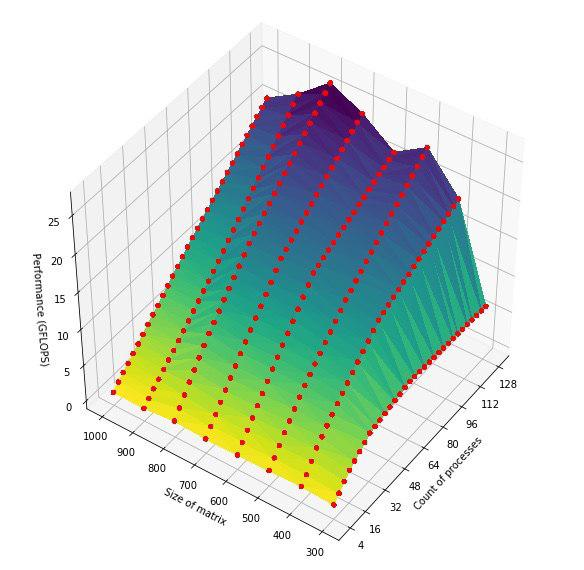
\includegraphics[scale=0.8]{image/p.jpg}
    \caption{Параллельная реализация алгоритма поиска автоморфизмов. Изменение производительности в зависимости от числа процессоров и размера матрицы.}
    \label{srg}
\end{figure}

\begin{figure}[ht]
\centering 
    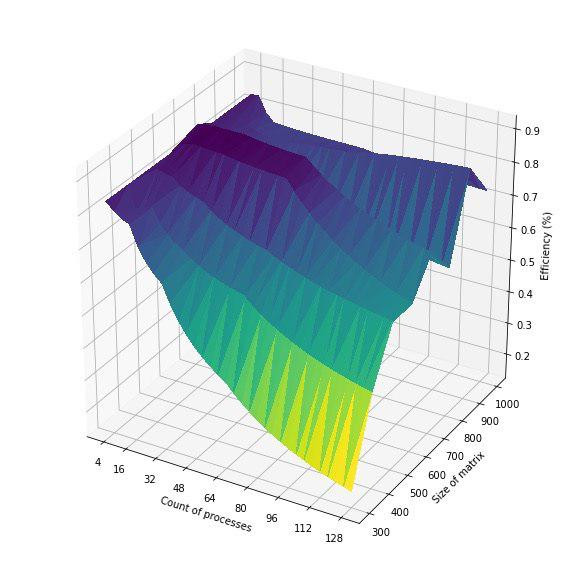
\includegraphics[scale=0.8]{image/ef.jpg}
    \caption{Параллельная реализация алгоритма поиска автоморфизмов. Изменение эффективности в зависимости от числа процессоров и размера матрицы.}
    \label{srg}
\end{figure}

Оценки масштабируемости выбранной реализации:
*	По числу процессов: -0,00837.
*	По размеру задачи: 0,04612. 
*	По двум направлениям: 0,00253.

 % результаты опробывания программ
\section*{Заключение}
\addcontentsline{toc}{section}{Заключение}
\label{sec:Conclusion} \index{Conclusion}
\large

\begin{itemize}
\item Выполнена модернизация алгоритма
\item Сформулировано утверждение вероятностной сложности алгоритма.

Разработан алгоритм с вероятностной сложностью:

$$O(n^2(\frac{e}{2})^{\ln(n)^2} \ln(n))$$

Алгоритм является универсальным и может применяться для решения большого количества задач (как минимум всех указанных в пункте 4.1 дипломной работы).

\item Реализовано 2 програмы: с графическим интерфейсом для удобного использования, с консольным интерфейсом для запуска на суперкомпьютере

Написанная программа с интерфейсом имеет масштабируемые функционал. На данный момент поддерживает функционал решения следующих задач (при $n \leq  500$):

\begin{itemize}
\item Поиск автоморфизмов
\item Поиск изоморфизмов
\item Поиск гомоморфизмов
\item Решение задачи Коши в подстановках
\end{itemize}

\item Проведены опыты на суперкомпьютере <<Ломоносов>>

Получены оценки сложности алгоритма при больших размерах графа (количество вершин $n$ > 1000).

\end{itemize}
 % заключение

\nocite{*}
\bibliographystyle{utf8gost71u}
\bibliography{References}

\section*{Приложение А}
\addcontentsline{toc}{section}{Приложение А}
\label{sec:Appendix_1} \index{Appendix_1}
\large

\begin{figure}[ht]
\centering 
    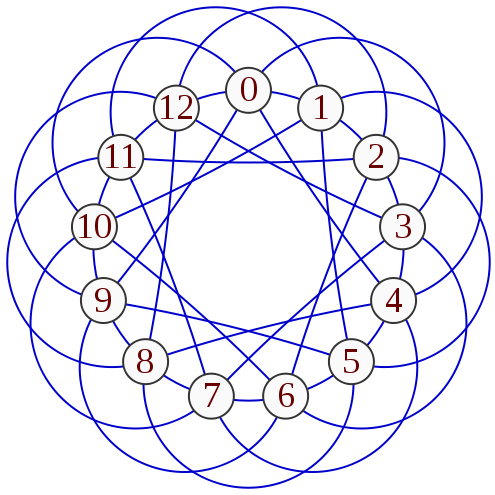
\includegraphics[scale=0.7]{image/srg_example.png}
    \caption{Граф Пейли 13-го порядка, сильно регулярный граф с параметрами srg(13,6,2,3).}
    \label{srg}
\end{figure}

\begin{figure}[H]
\centering
    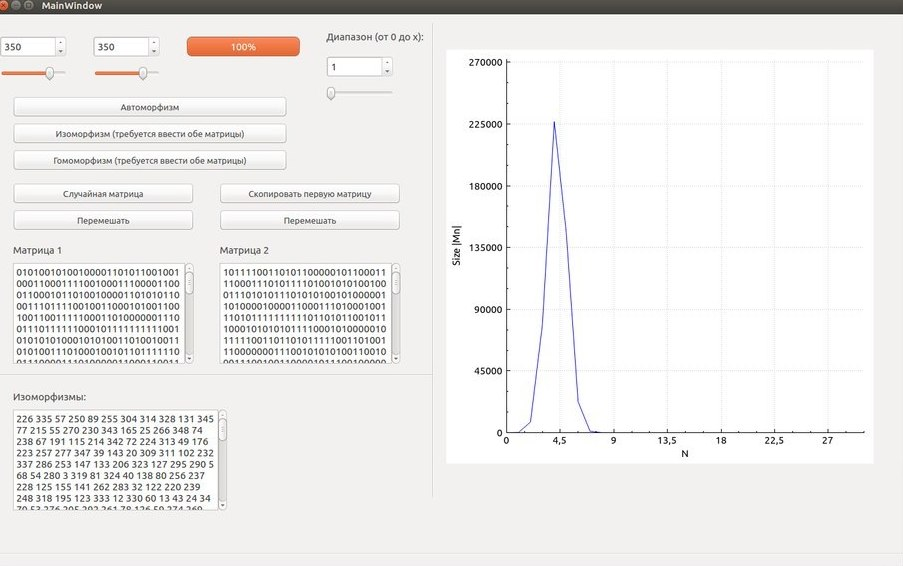
\includegraphics[scale=0.5]{image/program_example.jpeg}
    \caption{Примеры использования программы}
    \label{program_example}
\end{figure}

\begin{figure}[H]
\centering
	\begin{tikzpicture}[>=triangle 45,font=\sffamily]
    \node (X) at (0,0) {$M_0$};
    \node (Y) [below left=2cm and 1cm of X]  {$M_i$};
    \node (Z) [below right=2cm and 1cm of X] {$M_i$};
    \node (U) [below left=2cm and 1cm of Z]  {$M'_n$};
    \draw [semithick,->] (X) -- (Y);
    \draw [semithick,->] (X) -- (Z);
    \draw [semithick,->] (Y) -- (U) node [midway,below,sloped] {*};
    \draw [semithick,->] (Z) -- (U) node [midway,below,sloped] {*};
	\end{tikzpicture}
	\caption{Схема алгоритма}
	\label{algo_scheme}
\end{figure}

\begin{figure}[H]
\centering
	  \begin{tikzpicture}[domain=1:15, yscale=0.4, xscale=0.7] 
      \draw[step=3, very thin,color=gray] (-0.5,-0.5) grid (15.5,46.5);
      \draw[->] (0,0) -- (16,0) node[right] {$n$}; 
      \draw[->] (0,0) -- (0,47) node[above] {$f(n)$};
      \draw[color=red]    plot (\x,{pow(\x, 2) * pow(e/2, pow(ln(\x), 2)) * ln(\x)/300 })             node[right] {\Large $f(n) = n^2(\frac{e}{2})^{\ln(n)^2} \ln(n)$}; 
      \draw[color=blue]   plot (\x,{pow(e, sqrt(\x * log10(\x)))/20})    node[right] {\Large $f(n) = e^{\sqrt{n \times \log(n)}}$}; 
      \draw[color=blue] plot (\x,{pow(\x, pow(\x ,1/3) * pow(log10(\x), 2))/300}) node[right] {\Large $f(n) = n^{\O({n^{1/3}\log^{2} n})}$};
  	\end{tikzpicture}
	\caption{График сложности алгоритма}
	\label{algo_func}
\end{figure} % приложение
\section*{Приложение Б}
\addcontentsline{toc}{section}{Приложение Б}
\label{sec:Appendix_2} \index{Appendix_2}
\large 

Ссылка на дипломную работу с программой на github:\\
\href{https://github.com/fullincome/university}{https://github.com/fullincome/university}

Схема реализации представлена на языке C++

\begin{lstlisting}
#define GRAPH_SIZE 300
#define ROW_ARR_SIZE 10000 
#define COL_ARR_SIZE GRAPH_SIZE

const int N = GRAPH_SIZE;

vector<array<unsigned short,COL_ARR_SIZE>> 
Mi(ROW_ARR_SIZE, COL_ARR_SIZE);
vector<array<unsigned short,COL_ARR_SIZE>> 
M'i(ROW_ARR_SIZE, COL_ARR_SIZE);
unsigned char **matrix;

struct_M'i make_M'i(Mi) {
    struct_M'i M'i;
    for (auto x: Mi) {
        for (int i = 0; i < n; ++i) {
            if (check_h(x) && !eq(x, i)) {
                M'i.push_back(x.add(i));
            }
        }
    }
    return M'i;
}

struct_Mi make_Mi(M'i) {
    struct_Mi Mi;
    for (auto x: M'i) {
        for (int i = 0; i < n; ++i) {
           Mi.push_back(x.add(i));
        }
    }
    return Mi;
}

int main() {

    //fill matrix
    init_automorphisms(matrix);

    //parallelization of program
    switch(process) {
    case 0:
        begin = 0;
        end = stop_0;
    case 1:
        begin = start_1;
        end = stop_1;
    ...
    case N:
        begin = start_n;
        end = M_0.size();

    //main cycle
    for (i = begin; i < end; ++i) {
        Mi = make_Mi(M'i-1);
        M'i = make_M'i(Mi);
    }

    //results save (automorphisms output)
    final_automorphism(M'i);
}
\end{lstlisting}
 % приложение


\end{document}
